\subsection{Equilibrated MD}

Geometric analyses were performed to characterize the net molecular orientation of \wat~and \suldiox~molecules at different depths from the water surface location. At each distance from the surface location, an orientation profile was created for both the \wat~and \suldiox~molecules. The bivariate orientation distributions for the angles $\theta$ and $\phi$ at various depths were combined to form the intensity plots that show how the molecular orientation distributions change with distance to the surface location. These plots (Figures \ref{fig:water-orientation}, \ref{fig:so2-transit-angles}, and \ref{fig:so2-surface-angles}) allow for a visual interpretation of how the net orientations are affected when moving from the gas phase through the interfacial region and to the surface location, and then further into the aqueous interfacial region and bulk. Both the neat-water, with only a single \suldiox~introduced, and the high-concentration saturated system were analyzed. In the case of the neat-water system, the introduction of a single \suldiox~does not greatly affect molecular orientation of water molecules in the interfacial region. These results of the water orientation are very similar to a neat-water system without any adsorbed solutes (not shown).

The depth profile plots are arranged as a grid of 2D histograms. Each histogram is calculated for all molecules falling within a particular depth in the water interfacial region. The depth of each plot is marked (in \ang) in the upper-right, with the water surface location set at 0\angs, positive depths lie on the gas-phase side of the surface, and negative depths are on the bulk water side. The horizontal axes of each hisogram represent $\theta$ values, and the vertical axes represent $\phi$ values. Areas of low intensity appear in dark blue, and highest intensity in dark red. Regions of the plots where the intensity (coloration) is equally distributed along either the vertical or horizontal axes are considered isotropic in $\phi$ or $\theta$, respectively. Likewise, areas of the plot with high intensity over a small orientational range are considered to exhibit an orientational preference at the given depth. The angle distributions from both simulated slab surfaces were averaged for all the orientation analyses.

\subsubsection{\wat~Orientation}

The orientation depth-profiles for \wat~are shown in Figure \ref{fig:water-orientation} for both the neat-water (top) and saturated (bottom) systems during the equilibrium MD simulations. The interfacial region for both these calculations and the VSF experiments is defined as the region where molecular orientational anisotropy exists around the surface water location. Fitting the water density profiles we have calculated an interfacial width of approximately 10\angs~for the neat-water system, and approximately 16\angs~for the saturated system. In both systems the strongest orientational preference is found at the slab surfaces (positions near 0\angs). Previous work on orientational preference of water at air surfaces shows the same trend as our neat-water results.\cite{Walker2006b,Hore2008} The swaths of coloration indicating high intensity appearing in the neat-water plots from -4 to +4\angs, (and the corresponding regions in most of the saturated system plots) show the overall preference of water to orient at the surface. The plots of the neat-water and saturated systems are similar to each other with a narrow region of reorientation, but the effect in the interfacial region is greater in the neat-water system as evidenced by the sharper transition in intensity from blue to red, compared to the saturated system that has a less pronounced intensity change over larger areas of the histograms.

The bisector tilt of the water molecules, $\theta$, concentrates around $\theta=$ 90\textdegree within the first few\angs~above and below the water surface location, becoming progressively isotropic further through the interfacial region and into the water bulk of both systems. Above the surface location at positive distances, $\theta \leq$ 90\textdegree~indicates that the water hydrogens tend to point towards the gas-phase side of the surface. As the tilt nears $\theta=$ 90\textdegree~the \wat~bisector lies within the plane of the surface indicating a water orientation either flat on the surface, or with some amount of ``twist'' sending the OH bonds in towards, or out of the bulk. The value of $\phi$ determines the ``twist'' in this case. Both systems show a similar trend where waters at or just below the surface have values of $\phi$ near 90\textdegree, and waters above the surface take on values of $\phi$ near 0\textdegree. This jump in the angular distribution of $\phi$ indicates that waters at or below the surface lie mostly flat in the plane of the interface, and as they move above the surface towards the gas phase, they reorient with one OH bond pointing towards the water bulk, and one pointing out of the surface into the gas. This behavior is more strongly pronounced in the neat-water system where most of the surface waters are not interacting with an adsorbed layer of \suldiox~molecules.

%This result agrees somewhat with a recent air/water study by Fan et al. in which the surface orientations of several water models were analyzed.\cite{Fan2009} They simulated water using non-polarizable models, however, which alters the behavior of water at interfacial regions when compared to the polarizable POL3 model used in our work. The main conclusions are similar in that one OH tends to point further into the air phase than the other, but differs in that this effect is less pronounced with the polarizable model.

Although the plots show overall similarities for both the neat-water and saturated systems, the presence of a layer of adsorbed \suldiox~molecules alters the orientation of those waters furthest into the gas phase. For the saturated solution, the resulting orientation of waters above 0\angs, shown in the bottom plot of Figure \ref{fig:water-orientation}, is nearly isotropic in $\phi$, and with $\theta leq$ 90\textdegree. This results from waters with bisectors pointing further into the adsorbed \suldiox~gas layer, and both hydrogens pointing outward from the aqueous bulk. The effect is more pronounced as the waters move further from the water surface, and above 4\angs~the $\theta$ distribution is mostly centered around $\theta)=$ 0\textdegree (see Figure \ref{fig:water-angles}).

%The histograms show overall similarities for both systems in their shapes and intensities from approximately 0\angs~and below. The presence of a saturated layer of adsorbed \suldiox~molecules, however, alters the water orientation, but not necessarily the orientational depth of the interface. In both $\theta$ distributions, the orientations of waters in the bulk region are isotropic until 5\angs~below the surface location. At 5\angs~below the surface the water molecules begin to orient with their bisectors within the plane of the interface (perpendicular to the surface normal, $\cos(\theta)\approx 0$). The corresponding location in the plot of $\phi$ shows that those molecules are also mostly flat to the surface ($\cos(\phi)\approx 1$). Moving further out from the bulk and into the gas phase, the distributions show $\cos(\theta)$ increasing. Waters further out from the bulk have fewer bonding interactions, and orient with their hydrogens more towards the gas phase. The bisector pointing further into the gas phase leads to isotropy in the values of $\phi$.  

The angle distributions above 6\angs~in the neat-water plots of Figure \ref{fig:water-orientation} are mostly isotropic (manifested as uniform coloration throughout the range of orientations). Furthermore, there are few data points that make up the histograms, a result of fewer waters venturing beyond those extents. Conversely, waters near a layer of adsorbed \suldiox~venture further above the water surface location relative to the low \suldiox~concentration, where they can have interactions with the adsorbed \suldiox~gas molecules. The waters above the water surface location orient perpendicularly to the interface. This is consistent with our recent experimental VSFS studies which showed evidence for the reorienting behavior of water due to the \suldiox~interactions with the topmost surface waters.\cite{Ota2011}

The distribution of $\cos(\phi)$ is more sharply defined (i.e. less isotropic) for the neat-water system than for the saturated one. Waters on the neat surface lie flatter, whereas the presence of the \suldiox~allows a greater range of ``twist'' for those waters in the plane of the interface. The $\phi$ distributions quickly become isotropic above the surface location as the bisectors orient more perpendicularly, and below the surface as the bulk water loses any orientational preference.

%Peaks in the distributions of the neat-\wat~system are more clearly pronounced as their intensities are more concentrated and larger than the surrounding area of the profiles. This difference indicates that the transition from the preferred orientation at the water surface has a sharper distinction from the isotropic bulk than in the system with the saturated \suldiox~surface. It appears that the same orientation trend is present in both systems, but the presence of the \suldiox~at the water surface decreases the degree of water orientation at the interface.

\begin{figure}[h!]
	\begin{center}
		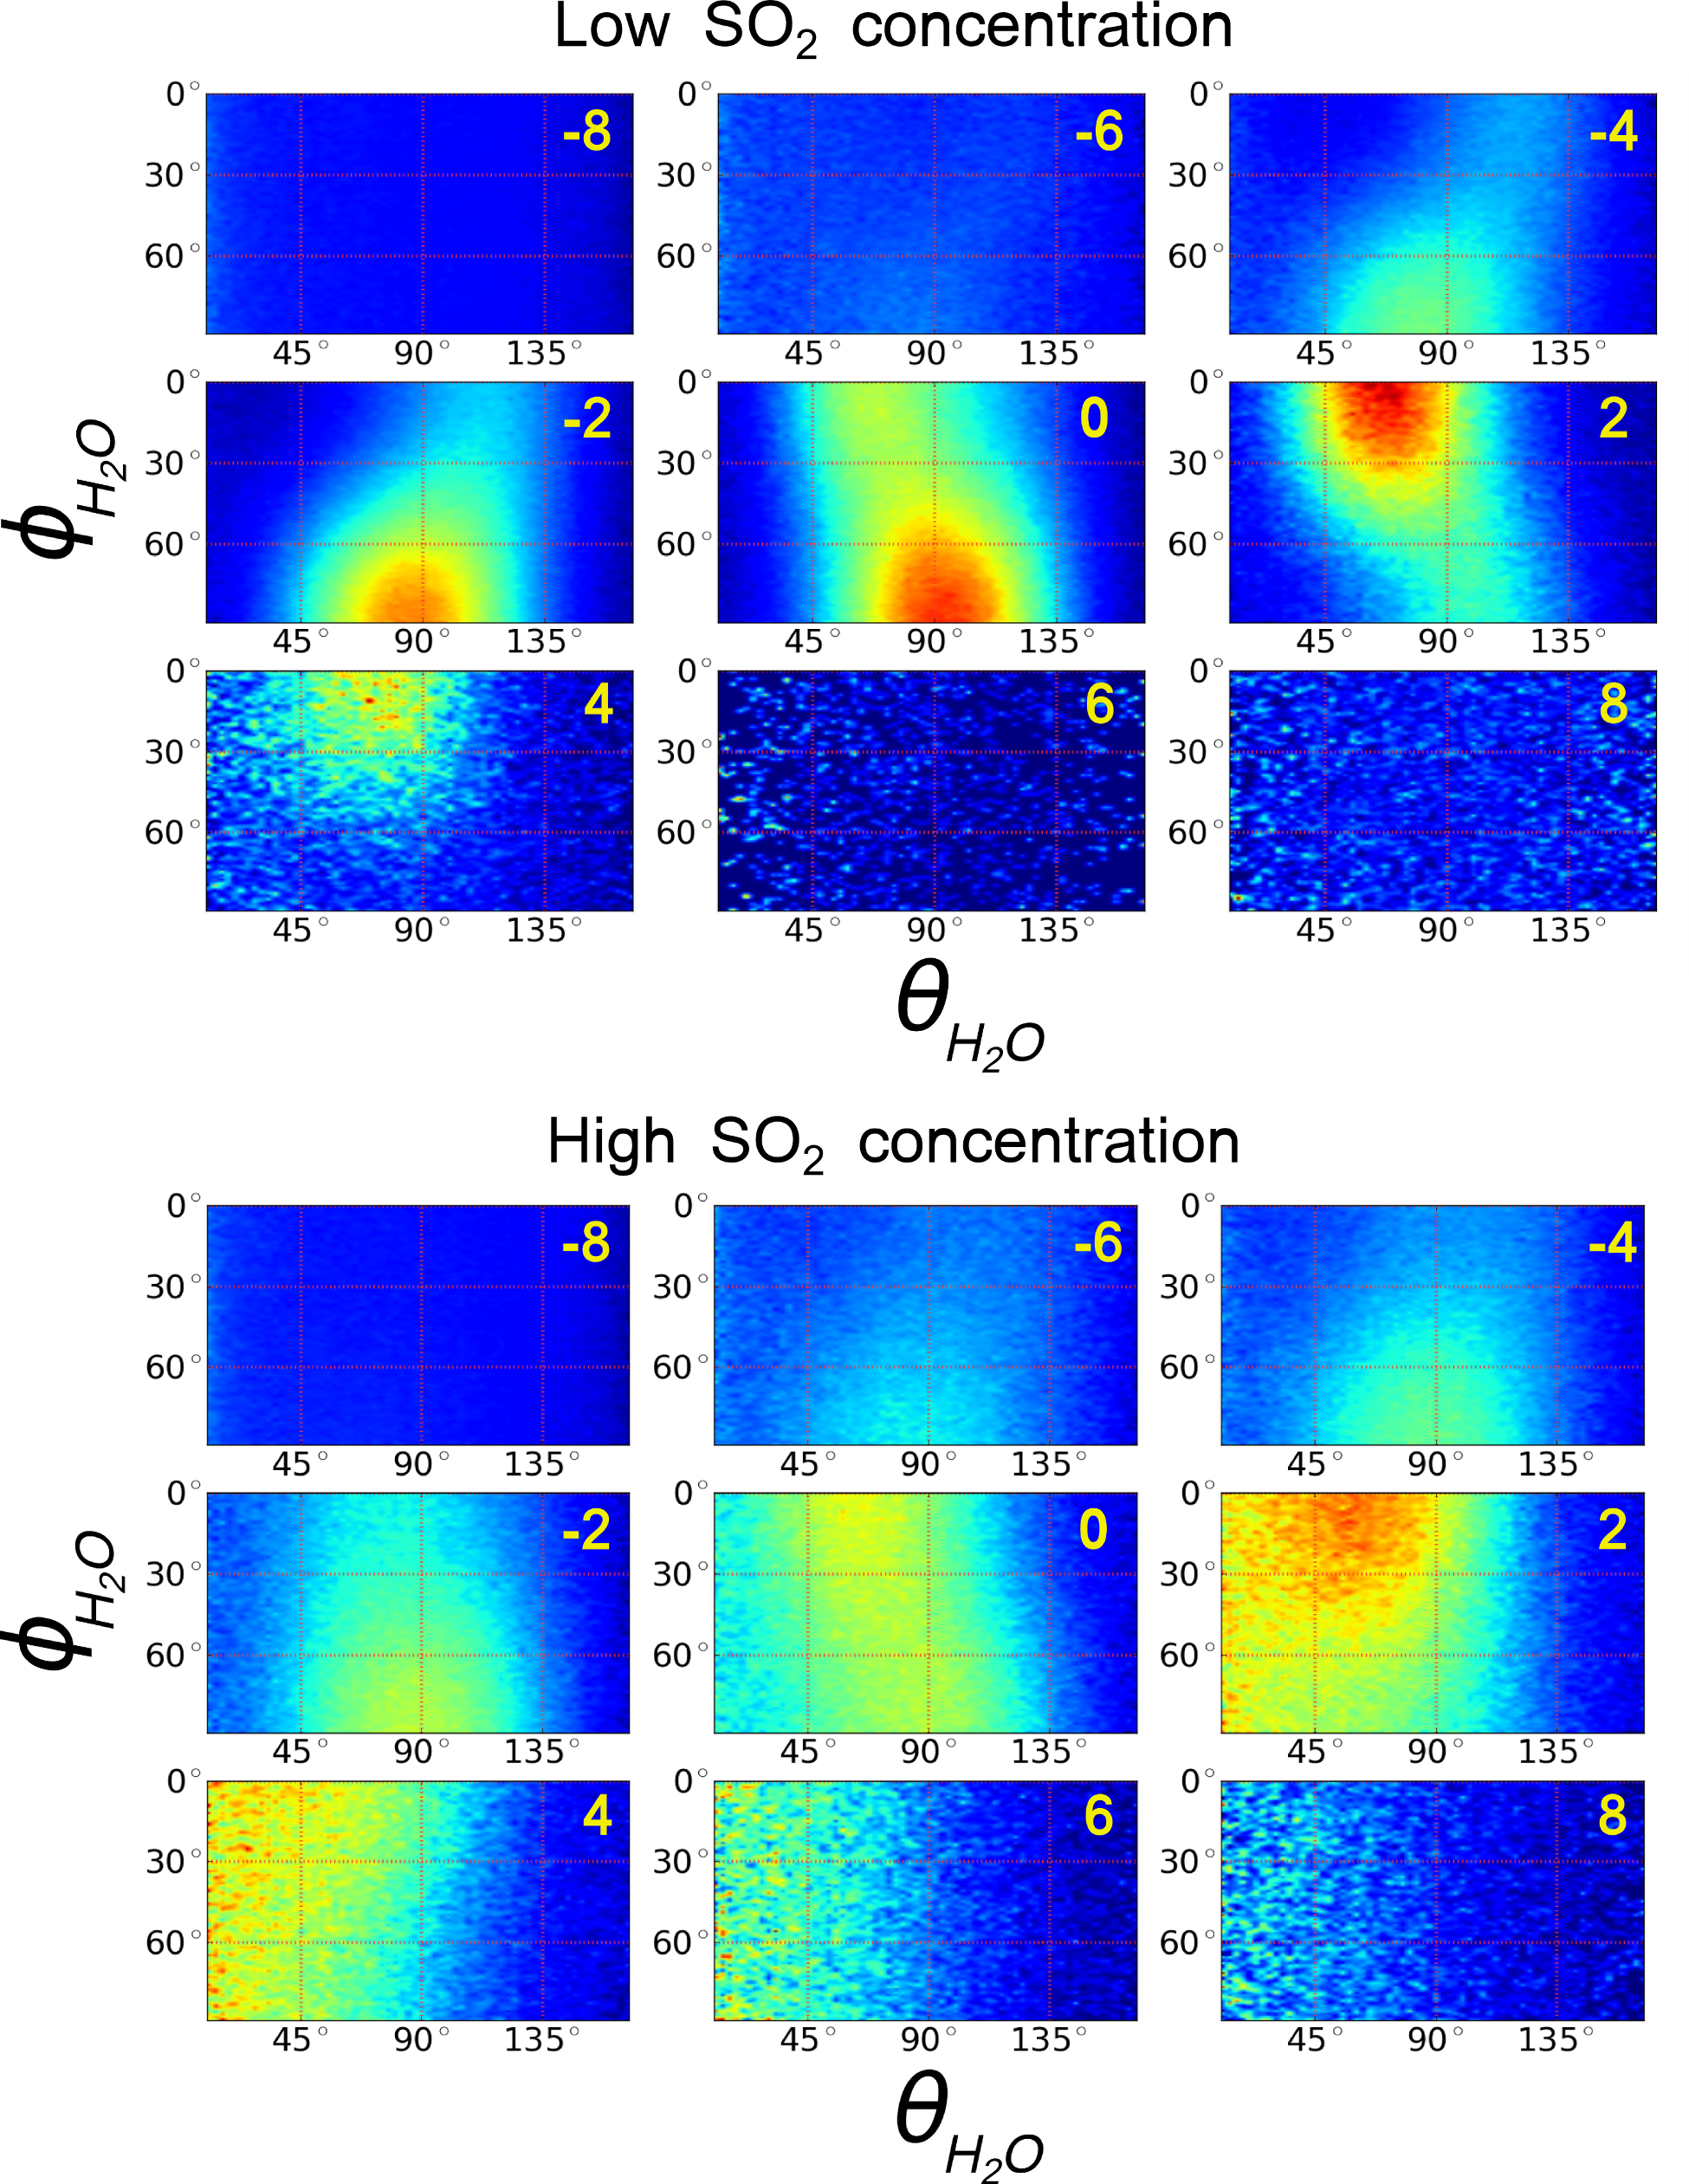
\includegraphics[scale=1.0]{images/h2o-angles/theta-phi.png}
		\caption{Molecular orientation histograms of \wat~throughout the surface equilibrated systems. The depth (in \angs) of each histogram within the water interface is numbered in the upper-right of each respective plot. The water surface location is set at a position of 0\angs~with negative distance values located in the bulk of the slab, and positive distances towards the gas phase. Each histogram is a bivariate angle distributions for $\theta$ (horizontal axes) and $\phi$ (vertical axes) in both the neat-\wat~system (top) and the saturated system (bottom). Regions of high intensity are dark red, and low intensity are dark blue.}
		\label{fig:water-orientation}
	\end{center}
\end{figure}


\subsubsection{\suldiox~Orientation}

Orientation distributions of the adsorbed \suldiox~molecules were created during the equilibrium simulations for both the neat-water and saturated systems. Figure \ref{fig:so2-orientation} shows the 2D distributions of $\theta$ and $\phi$ (arranged similarly to the water orientation distributions plots in Figure \ref{fig:water-orientation}). The \suldiox~orientation data set for the neat-water system is much smaller as only a single \suldiox~molecule was simulated in the bulk. The resulting distribution plots are thus representative of the single surface active \suldiox~molecule. The neat-water \suldiox~molecule remains within a narrower region of the interface than the saturated system \suldiox, but effective comparisons can still be drawn.

In the interfacial region the angular distribution of the single \suldiox~(in the neat-water system) is concentrated primarily in $\theta <$ 90 \textdegree. The peak of the distribution occurs at $\theta)=$ 0\textdegree. This indicates that the \suldiox~bisector points out of the water surface, with the sulfur atom pointing towards the aqueous bulk, and the two oxygens pointing into the gas phase. This same distribution occurs in the saturated system for depths below the surface location, $< 0$\angs. Beyond 4\angs~above the surface, both distributions become mostly isotropic, either because the \suldiox~does not venture into the gas in the neat-water system, or because of the nature of the adsorbed \suldiox~layer in the saturated system. Promixity to the water surface highly orients the \suldiox~bisector. % with the sulfur atom pointing in towards the water bulk. %Moving further away from the water surface, and interacting less with \wat~molecules allows for greater orientational freedom as exhibited in the isotropy of the distributions above 4\angs. %Because both the neat-water and saturated systems show rather similar distributions, it is possible that the concentration of \suldiox~does not strongly affect the orientation of the \suldiox, unlike the orientations of waters.

The distributions of $\phi$ are isotropic in both systems at all depths. Because the \suldiox~bisector near the surface is oriented perpendicularly to the interface, the isotropy in $\phi$ is expected. Further from the water surface where the bisector orientation becomes isotropic, the $\cos(\phi)$ distribution remains isotropic. For the \suldiox~orientation, the $\phi$ angle does not provide further information regarding the surface behavior or orientational preference.

%The plots indicate that \suldiox~orients similarly at both the low and high concentration interfacial environments. The $\theta$ values follow similar trends at both concentrations indicating that the \suldiox~sulfur orients down towards the water phase, with both oxygens pointing away from the surface once the \suldiox~is within approximately 5\angs~of the surface. This behavior continues down to at least 5\angs~below the water surface location, notwithstanding any chemical reactions that may occur that are not simulated using the classical MD techniques utilized in this work.

\begin{figure}[h!]
	\begin{center}
		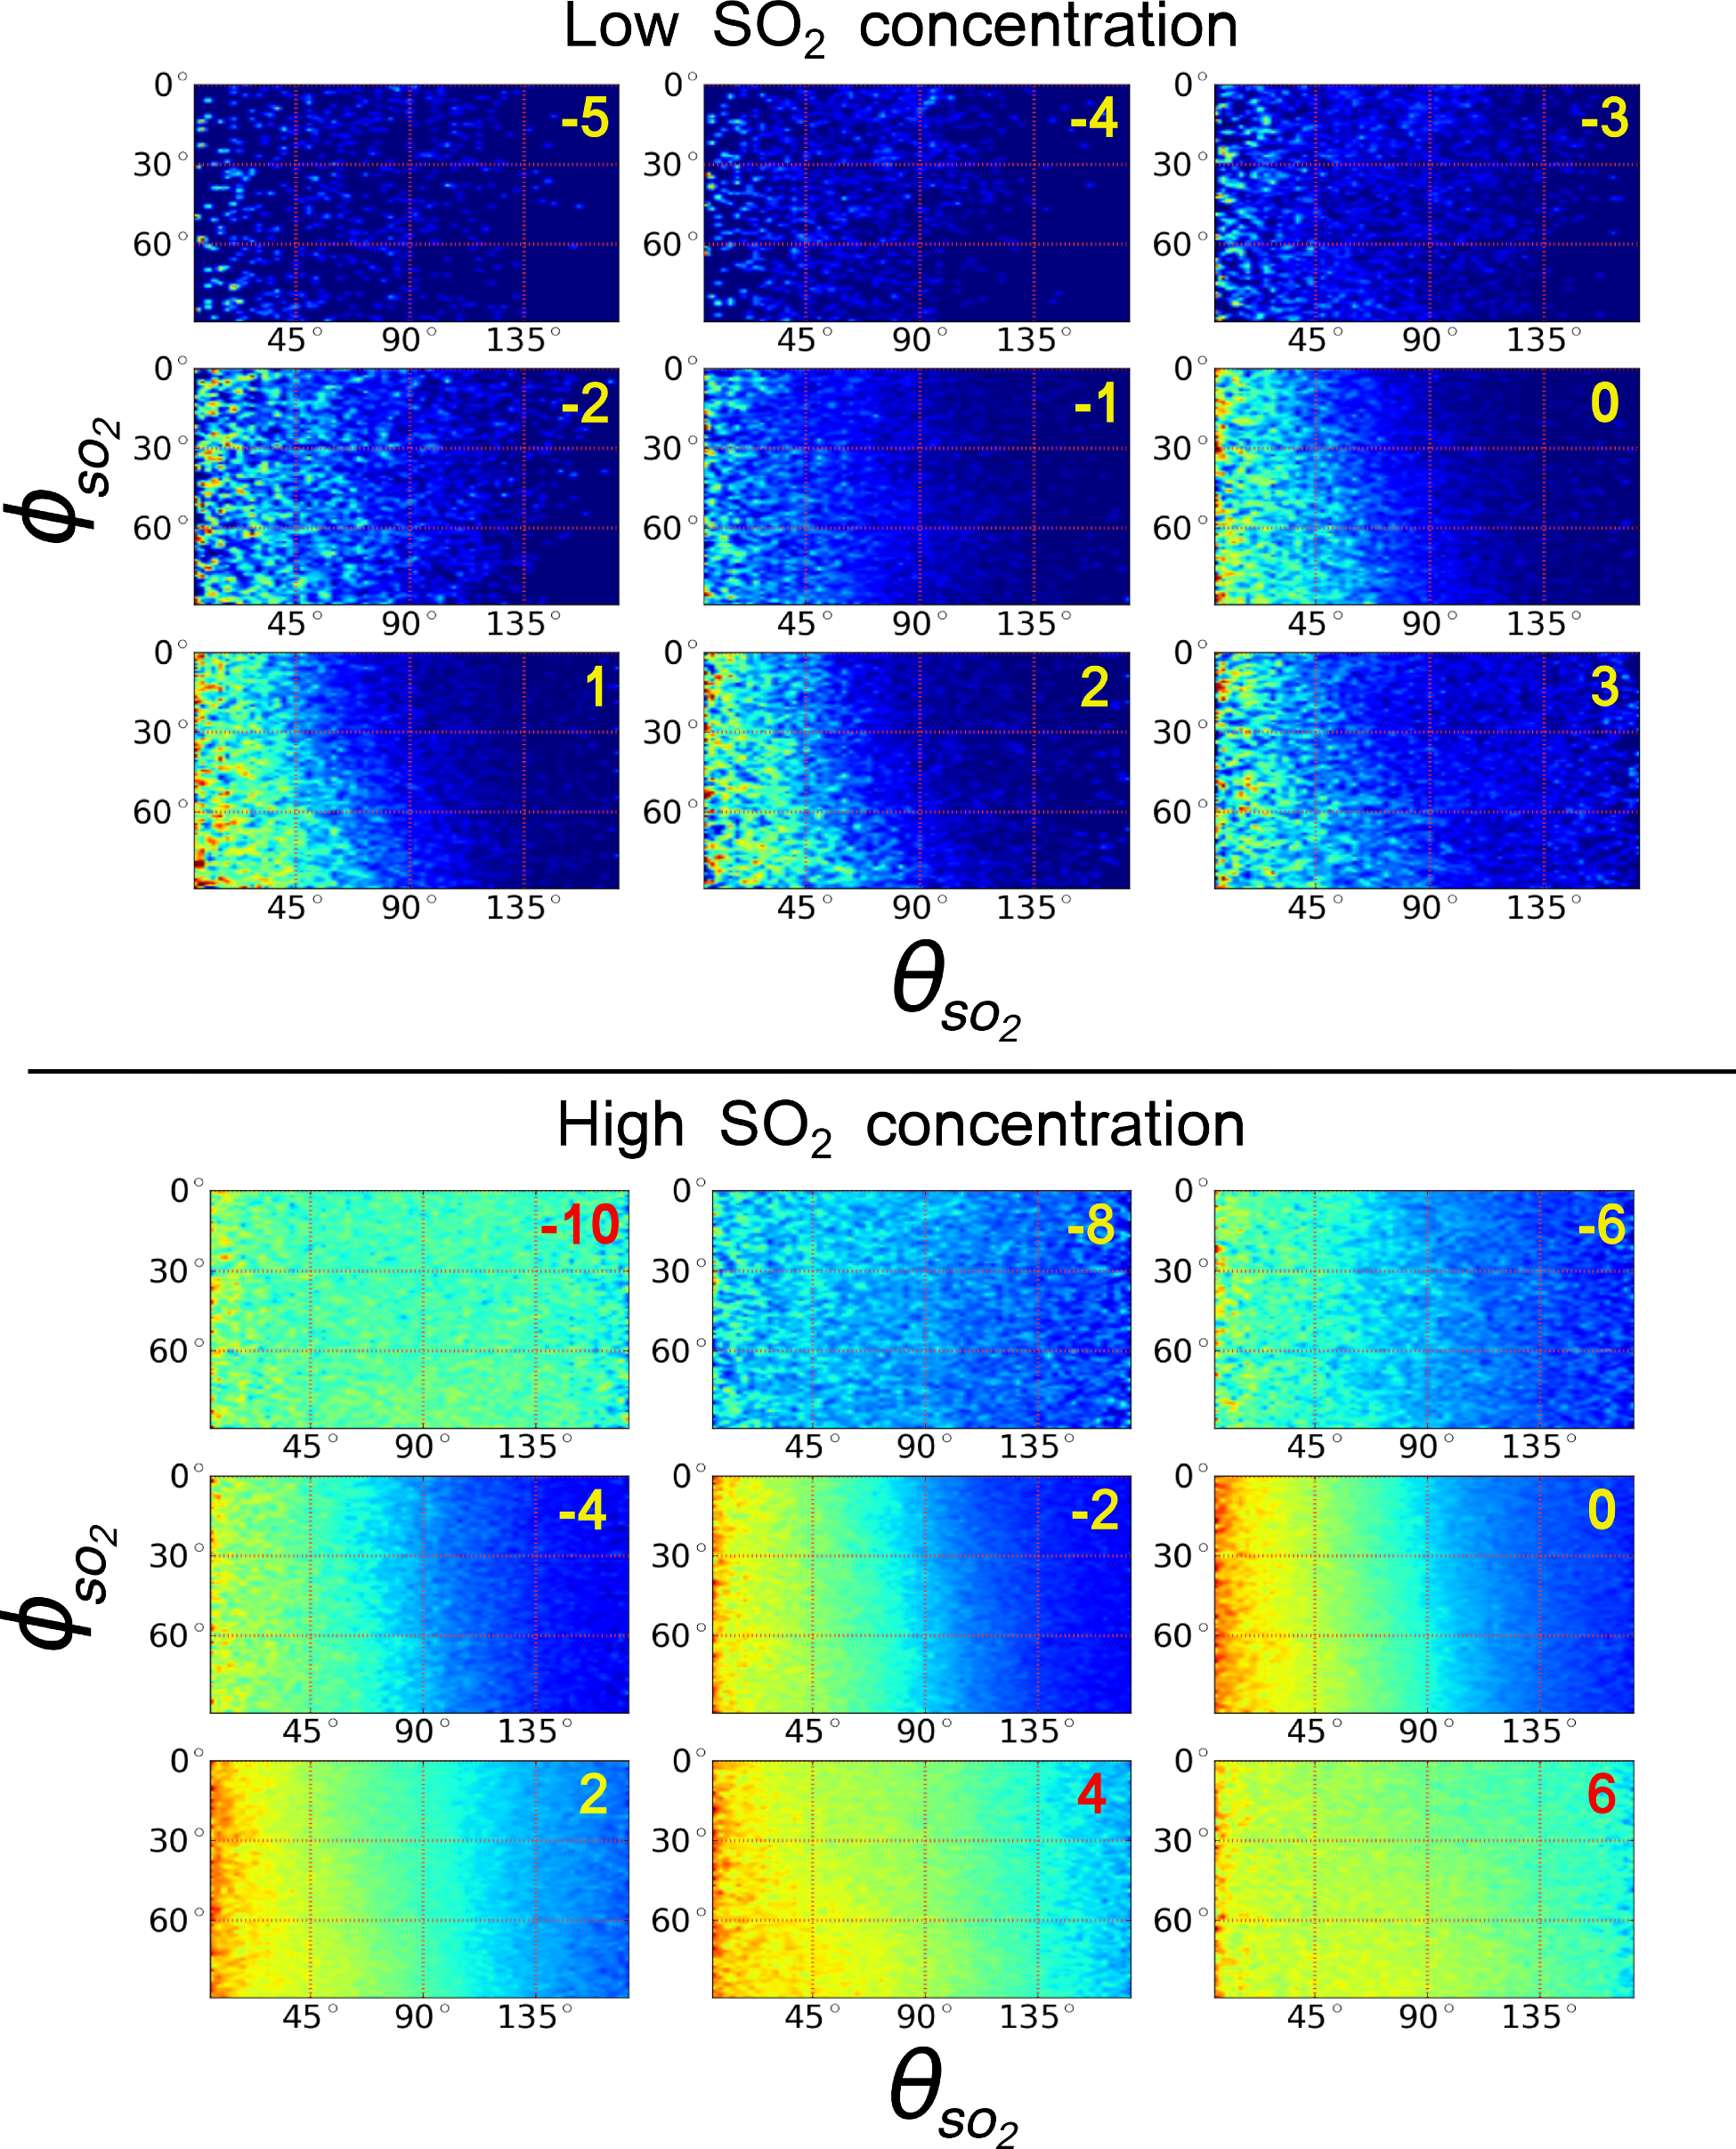
\includegraphics[scale=1.0]{images/so2-angles/theta-phi.png}
		\caption{Molecular orientation distributions for \suldiox~molecules adsorbed to the water slab surface. The angular distributions are shown for the neat-water (top) and saturated (bottom) systems, and are arranged similarly to the water orientation plots of Figure \ref{fig:water-orientation}. For both systems the distributions show \suldiox~bound to the water surface with the sulfur primarily pointing towards the water slab, and the oxygens pointing to the gas phase. In this configuration the $\phi$ distribution is isotropic because of the water slab's in-plane symmetry. Note that the range of surface depths in the low concentration system is half that of the saturated system. This is due to the narrower position range of the single \suldiox~molecule.}
		\label{fig:so2-orientation}
	\end{center}
\end{figure}
